% ------------ begin cheatsheet
\documentclass[a4paper]{article}
\usepackage[a4paper,margin=0.03in]{geometry}
\usepackage{multicol}

\usepackage{amsmath, amssymb}
\usepackage[inline]{enumitem}
\usepackage{graphicx}
\usepackage{xcolor}

\usepackage{ulem}
\usepackage{makecell}

% math-mode version of "c" column type
\newcolumntype{C}{>{$}c<{$}}

\newcommand{\Z}{\mathbb{Z}}

% horizontal list
\newlist{hlist}{enumerate*}{1}
\setlist[hlist]{label={}, afterlabel={}, itemjoin={{ \textbar{} }}}

% math
\newcommand{\abs}[1]{\left\lvert#1\right\rvert}
\usepackage{spalign}
\let\mat=\spalignmat
\let\amat=\spalignaugmat
\newcommand{\pp}{{\prime\prime}}
\newcommand{\sgn}[1]{\mathrm{sgn}(#1)}
\newcommand{\gen}[1]{\langle #1 \rangle}
\newcommand{\ord}[1]{\mathrm{o}(#1)}
\newcommand{\kernel}[1]{\mathrm{ker} \; #1}
\newcommand{\sub}[1]{\mathrm{\textbf{Sub}}(#1)}
\newcommand{\Aut}[1]{\mathrm{Aut}(#1)}
\newcommand{\Inn}[1]{\mathrm{Inn}(#1)}
\newcommand{\vv}{\vert\vert}

% envs
\newcommand{\oli}[1]{\begin{enumerate*}[label=(\arabic*)]#1\end{enumerate*}}
\newcommand{\yellow}[1]{\colorbox{yellow}{#1}}

\graphicspath{ {./images/} }
\pagestyle{empty}
\setlength{\columnseprule}{0.2pt}

% reduce spacing before and after headers
\newcommand{\uppercaseandunderline}[1]{\uline{\uppercase{#1}}}

\makeatletter
\renewcommand{\section}{
  \@startsection{section}{1}{0pt}{1ex}{1.2ex} {\raggedleft\normalfont\large\bfseries\uppercaseandunderline}}
\renewcommand{\subsection}{
  \@startsection{subsection}{2}{0pt}{1ex}{1.2ex} {\raggedleft\normalfont\normalsize\bfseries\fbox}}
\renewcommand{\subsubsection}{
  \@startsection{subsubsection}{3}{0pt}{1ex}{0.8ex} {\raggedleft\normalfont\footnotesize\bfseries\uline}}
\renewcommand{\paragraph}{
  \@startsection{paragraph}{4}{0pt}{1.5ex}{-0.8em}{\normalfont\bfseries}}
% ------------ end cheatsheet

\begin{document}
\footnotesize
\setlength{\abovedisplayskip}{2pt}
\setlength{\belowdisplayskip}{2pt}
\setlength{\abovedisplayshortskip}{0pt}
\setlength{\belowdisplayshortskip}{0pt}
\begin{multicols*}{3}
  \section*{\centering \underline{MA2202}}
  \subsubsection*{Fermat's little theorem} \noindent
  Let $p$ be a prime number. Then
  \[ p|(n^p - n) \quad \forall n \in \Z \]
  i.e.
  \[ n^p \equiv n \pmod{p} \implies n^{p-1} \equiv 1 \pmod{p} \]
  Applying this idea,
  \[ n^{a(p-1)+b} \equiv n^b \pmod{p} \]
  \subsection*{Group isomorphisms}
  \subsubsection*{Definition} \noindent
  If $G \cong H$:
  \begin{itemize}[leftmargin=*]
    \item If $G$ is abelian, $H$ is abelian.
    \item $\phi: G \rightarrow G$ given by $\phi(g) = g^{-1}$ is a group isomorphism $\iff G$ is an abelian group.
  \end{itemize}
  \subsubsection*{Two isomorphisms} \noindent
  Suppose $\phi: (G,*) \rightarrow (H,\star)$ and $\psi: (H, \star) \rightarrow (K, \cdot)$ are two isomorphisms of groups. Then
  \begin{itemize}[leftmargin=*]
    \item the inverse function $\phi^{-1}: (H,\star) \rightarrow (G,*)$ and
    \item the composite function $\psi \circ \phi: (G,*) \rightarrow (K,\cdot)$
  \end{itemize}
  are group isomorphisms.
  \subsection*{Subgroups}
  \paragraph{Roots of unity} $(\mu_m, \times)$ is a subgroup of $(\mu_n, \times)$ if $m \vert n$.
  \begin{itemize}
    \item   Let $(G,*)$ be a group and let $H \subseteq G$ be a nonempty subset. Then $(H,*)$ is a subgroup iff for all $a,b \in H$, we have $a * b^{-1} \in H$.
    \item Intersection of a finite collection of subgroups is a non-empty subgroup.
    \item   Let $(H,*)$ and $(K,*)$ be subgroups of $(G,*)$. If $(H \cup K, *)$ is a subgroup, then either $H \subseteq K$ or $K \subseteq H$.
  \end{itemize}
  \subsection*{Cyclic notations} \noindent
  Fix $f \in S_n$. Let $x \in X = \{1, \cdots, n\}$. Consider the sequence of integers in $X$: $x_0, x_1, x_2, \cdots$, where $x_0 = x$ and $x_i = f^i(x) \in X$.
  \begin{itemize}[leftmargin=*]
    \item Since $X$ is finite, the sequence will repeat. Let $x_r$ be the first integer that repeats in the sequence. Can be shown that $x_r = x_0 = x$.
    \item $\mathcal{O} = \{x_0, x_1, \cdots, x_{r-1}\}$ is an orbit of the powers of $f$.
    \item The sequence $(x_0 x_1 \cdots x_{r-1})$ is called a cycle.
    \item $X = \bigsqcup_j \mathcal{O}_j$
  \end{itemize}
  \paragraph{Example} $f = (16)(24)(3789)(5)$
  \begin{itemize}[leftmargin=*]
    \item $f$ is also equal to $(61)(24)(8937)(5)$. We can rotate within the cycle.
    \item $f$ is also equal to $(16)(24)(3789)$. We can drop singleton cycles.
    \item $h = (16)$ is the bijection in $S_9$ such that $h(1) = 6, h(6) = 1$ and $h(x) = x$ for $x \ne 1, 6$.
    \item $f$ is also equal to $(24)(16)(3789)(5)$. We can swap the cycles because they represent bijections in $S_9$ which are disjointed cycles and they are commutative.
  \end{itemize}
  \paragraph{Cyclic permutation}
  A bijection $h \in S_n$ which is represented by a single cycle is called a cyclic permutation or cycle. Two cycles
  \[ h = (i_1 \cdots i_r) \text{ and } h' = (j_1 \cdots j_s) \]
  are called disjointed cycles if $i_\alpha \ne j_\beta$ for all $\alpha = 1, \cdots, r$ and $\beta = 1, \cdots, s$.
  \paragraph{Theorem 23}
  Let $f \in S_n$. Then
  \begin{itemize}[leftmargin=*]
    \item $f = h_1 \circ h_2 \circ \cdots \circ h_r$ can be factorized into a product of mutually disjointed cycles.
    \item The factorization is unique up to an ordering of the product of cycles, i.e. if
          \[ f = h_1 \circ h_2 \circ \cdots \circ h_r = k_1 \circ k_2 \circ \cdots \circ k_s \]
          are two factorization into mutually disjointed cycles, then by renaming the cycles $k_i$ if necessary, we have $r = s$ and $h_i = k_i$ for $i = 1, \cdots, r$.
  \end{itemize}
  \paragraph{Transpositions}
  A cycle $h \in S_n$ of the form $h = (ij)$ is a transposition.
  \begin{itemize}[leftmargin=*]
    \item $(i_1 i_2 \cdots i_r) = (i_1 i_r)(i_1 i_{r-1}) \cdots (i_1 i_2)$. Hence, a cycle is a product of transpositions.
    \item Since $f \in S_n$ is a product of cycles, $f$ is also a product of transpositions.
  \end{itemize}
  \subsection*{The sign character}
  \paragraph{Lemma} For all permutation matrices $F, H \in S_n^\pp$,
  \begin{itemize}[leftmargin=*]
    \item $\det(F) = \det(F^T) = \pm 1$.
    \item $\det(FH) = \det(F) \det(H)$.
  \end{itemize}
  \paragraph{Proposition 25}
  Let $P(\boldsymbol{x}) = P(x_1, \cdots, x_n) = \displaystyle \prod_{1 \le i < j \le n} (x_i - x_j)$. For $f \in S_n$, let
  \begin{align*}
    P_f(\boldsymbol{x}) & = P_f(x_1, \cdots, x_n) = P(x_{f(1)}, \cdots, x_{f(n)}) \\
                        & = \prod_{1 \le i < j \le n} (x_{f(i)} - x_{f(j)})
  \end{align*}
  \begin{itemize}[leftmargin=*]
    \item $P_f(\boldsymbol{x}) = P(\boldsymbol{x})$ or $-P(\boldsymbol{x})$. We write $P_f(\boldsymbol{x}) = \sgn{f} P(\boldsymbol{x})$, where $\sgn{f} = \pm 1$.
    \item $\sgn{f \circ h} = \sgn{f} \sgn{h}$.
  \end{itemize}
  \paragraph{Even/odd} Let $f, h \in S_n$.
  \begin{itemize}[leftmargin=*]
    \item $f$ is an even permutation if $\sgn{f} = 1$, and odd if $\sgn{f} = -1$.
    \item If $f$ and $h$ are both even (odd), then $f \circ h$ is even (odd).
    \item If $f$ is odd and $h$ is even, then $f \circ h$ is odd.
    \item A transposition is an odd permutation.
    \item A product of an even (odd) number of transpositions is even (odd).
    \item $f$ is even $\iff f$ is a product of an even number of transpositions.
  \end{itemize}
  \paragraph{Alternating group} Let
  \[ A_n = \{f \in S_n: \sgn{f} = 1\} = \{f \in S_n: f \text{ even}\} \]
  be the set of all even permutations in $S_n$. Then $(A_n, \circ)$ is a subgroup of $(S_n, \circ)$.
  \begin{itemize}[leftmargin=*]
    \item The subset of odd permutations is not a subgroup.
  \end{itemize}
  \subsection*{Cayley's theorem} \noindent
  Let $(G,\ast)$ be a finite group of order $n$. Then $(G,\ast)$ is isomorphic to a subgroup of $(S_n,\circ)$.
  \subsubsection*{Proof}
  \begin{itemize}[leftmargin=*]
    \item We know that $(S_Y,\circ)$ is isomorphic to $(S_n,\circ)$.
    \item Let $Y=G$. For every $g \in G$, define function $f_g: Y \rightarrow Y$ by
          \[ f_g(y) = g \ast y \text{ for all } Y = G \]
          Then construct $\phi: G \rightarrow S_Y$ by $\phi(g) = f_g$. $\phi$ is an injective group homomorphism, so $G$ is isomorphic to the image $G'$ which is a subset of $S_Y$, i.e. $G$ is isomorphic to a subgroup of $(S_Y, \circ)$.
  \end{itemize}
  \subsection*{Cosets and Lagrange's theorem}
  \subsubsection*{Coset} \noindent
  Let $H$ be a subgroup of $G$. For $g \in G$, denote
  \[ gH = \{gh: h \in H\} \text{ and } Hg = \{hg: h \in H\} \]
  These are called a left coset and a right coset of $H$ in $G$ respectively. Note that $eH = He = H$.
  \begin{itemize}[leftmargin=*]
    \item If $G$ is abelian, then a left coset is also a right coset.
  \end{itemize}
  \subsubsection*{Mutually disjointed subsets} \noindent
  Let $S$ be a set, and let $\{S_i: i \in I\}$ be a collection of subsets of $S$.
  \begin{itemize}[leftmargin=*]
    \item We say that $\{S_i: i \in I\}$ is a collection of mutually disjointed subsets if $S_i \cap S_j = \emptyset$ for every distinct $i, j \in I$.
    \item We say that $\{S_i: i \in I\}$ forms a partition of $S$ if it is a collection of mutually disjointed subsets, and $S = \bigcup_{i \in I} S_i$. We write $S = \prod_{i \in I} S_i$.
  \end{itemize}
  \subsubsection*{Proposition 37} \noindent
  Let $G$ be a group and let $H$ be a subgroup. Let $x, y, z \in G$.
  \begin{enumerate}[label=\roman*., leftmargin=*]
    \item If $z \in xH$, then $zH = xH$.
    \item If $xH \cap yH \ne \emptyset$, then $xH = yH$.
    \item The collection of left cosets $\{xH: x \in G\}$ forms a partition of $G$.
    \item Every coset $xH$ is of the same cardinality as $H$, i.e. there is a bijection $f: H \rightarrow xH$. If $H$ is a finite group, then $\abs{H} = \abs{xH}$.
  \end{enumerate}
  \subsubsection*{Definition}
  \begin{itemize}[leftmargin=*]
    \item Denote $G/H = \{xH: x \in G\}$ and $H \backslash G = \{Hx: x \in G\}$.
    \item Let $[G:H]$ denote the number of distinct left cosets of $H$ in $G$, i.e. $[G:H] = \abs{G/H}$. It is called the index of $H$ in $G$.
  \end{itemize}
  \subsubsection*{Lagrange's Theorem} \noindent
  Let $G$ be a finite group and let $H$ be a subgroup.
  \begin{itemize}[leftmargin=*]
    \item $\abs{H}$ divides $\abs{G}$.
    \item $[G:H] = \abs{G/H} = \abs{G} / \abs{H}$.
    \item $[H:G] = \abs{H\backslash G} = \abs{G} / \abs{H}$.
  \end{itemize}
  \paragraph{Corollary} Let $p$ be a prime integer, and let $G$ be a group of order $p$.
  \begin{itemize}[leftmargin=*]
    \item The only subgroups of $G$ are $\{e\}$ or $G$.
    \item Let $x \in G$ and $x \ne e$. Let $x = \gen{x} = \{x^n: n \in \Z\}$ be the cyclic subgroup of $G$ generated by $x$. Then $G = \gen{x}$.
  \end{itemize}
  \paragraph{Corollary} If $H$ is a subgroup of $G$ and $K$ is a subgroup of $H$, then
  \[ [G:K] = [G:H][H:K] \]
  \subsection*{Generators}
  \paragraph{Subgroup}
  Let $G$ be a group, and let $X \subseteq G$. Let $S = \{H: H \text{ subgroup of } G, H \supseteq X\}$. We define
  \[ \gen{X} = \bigcap_{H \in S} H \]
  and we call $\gen{X}$ the subgroup of $G$ generated by $X$.
  \begin{itemize}[leftmargin=*]
    \item If $H$ is a subgroup of $G$ containing $X$, then by definition, $H$ contains $\gen{X}$. Hence, $\gen{X}$ is also called the smallest subgroup of $G$ containing $X$.
    \item If the subgroup $\gen{X} = G$, then we say that $G$ is generated by $X$.
    \item We say that a group $G$ is finitely generated if it is generated by some finite subset. $G$ could still be infinite, e.g. $G = (\Z, +)$ is generated by $X = \{1\}$.
  \end{itemize}
  \paragraph{Word}
  A word on $X$ is either $e$ or a finite product $x_1^{r_1} x_2^{r_2} \cdots x_n^{r_n} \in G$ where $x_i \in X$ and $r_i \in \Z$ for $i=1, \cdots, n$.
  \begin{itemize}[leftmargin=*]
    \item Some $x_i$ can be the same.
    \item Some $r_i$ may be negative integers.
    \item If $G$ is non-abelian, order of multiplication matters.
    \item Two different words may represent the same element in $G$.
  \end{itemize}
  \subsubsection*{Proposition 39} \noindent
  Let $X$ be a subset of a group $G$. Let $W$ be the set of words on $X$. Then $W$ is a subgroup and $W = \gen{X}$.
  \subsection*{Cyclic groups}
  \paragraph{Proposition} Let $(G, \ast)$ be a group. Pick $a \in G$. The subset $\gen{a} = \{a^n \in G: n \in \Z\}$ is a subgroup of $(G, \ast)$. It is called the cyclic subgroup of $G$ generated by $a$.
  \begin{itemize}[leftmargin=*]
    \item $\gen{a} = \gen{a^{-1}}$.
  \end{itemize}
  \paragraph{Proposition 40} The order of the subgroup $\abs{\gen{a}}$ is equal to the order $\ord{a}$.
  \paragraph{Proposition 41} Let $G$ be a finite group. Let $a \in G$. Then $\ord{a}$ divides $\abs{G}$.
  \paragraph{Corollary 42} Let $G$ be a finite group of order $p$ where $p$ is a prime number. Pick $a \in G$ and $a \neq e$. Then
  \[ G = \gen{a} = \{e, a, \cdots, a^{p-1}\} \]
  \subsubsection*{Cyclic group} \noindent
  Let $(G,*)$ be a group and let $x \in G$. A group $(G,*)$ is called a cyclic gp if $G = \gen{x}$ for some $x \in G$, i.e.
  \[ G = \gen{x} = \{x^n \in G : n \in \Z\} \]
  \begin{itemize}[leftmargin=*]
    \item Group $G$ is cyclic $\implies$ some element $x \in G$ has order $\abs{G}$
  \end{itemize}
  \subsection*{Group homomorphisms} \noindent
  Let $(G,*)$ and $(H,\star)$ be two groups. A function $\phi: G \rightarrow H$ is called a group homomorphism if
  \[ \phi(x*y) = \phi(x) \star \phi(y) \]
  for all $x,y \in G$.
  \begin{itemize}[leftmargin=*]
    \item There is no requirement on $\phi$ to be injective or surjective. But if $\phi$ is a bijection, then we have a group isomorphism instead.
    \item Composition of group homomorphisms is a group homomorphism.
    \item Let $\phi: (G,\ast) \rightarrow (H,\star)$ be an injective group homomorphism. Then $(G,\ast)$ is isomorphic to its image which is a subgroup of $(H,\star)$.
  \end{itemize}
  \paragraph{Proposition 43} Let $\phi: (G,\ast) \rightarrow (H,\star)$ be a group homomorphism.
  \begin{enumerate}[label=\roman*., leftmargin=*]
    \item Let $e_G$ and $e_H$ be identity elements of the groups $G$ and $H$ respectively. Then $\phi(e_G) = e_H$.
    \item For all $g \in G$, $\phi(g^{-1}) = (\phi(g))^{-1}$.
    \item Let $G'$ be a subgroup of $G$. Then the image $\phi(G')$ is a subgroup of $H$.
    \item Let $H'$ be a subgroup of $H$. Then $\phi^{-1}(H')$ is a subgroup of $G$.
  \end{enumerate}
  \paragraph{Kernel} Let $\phi: (G,\ast) \rightarrow (H,\star)$ be a group homomorphism. The kernel of $\phi$ is defined as
  \[ \kernel{\phi} = \phi^{-1}(e_H) = \{g \in G: \phi(g) = e_H \} \]
  It is the set of elements in $G$ that is sent to $e_H$ under the mapping $\phi$.
  \paragraph{Prop. 44} Let $\phi: (G,\ast) \rightarrow (H,\star)$ be a group homomorphism and let $K$ be the kernel of $\phi$.
  \begin{enumerate}[label=\roman*., leftmargin=*]
    \item The kernel $K$ is a subgroup of $G$.
    \item $\forall g_0 \in K$ and $g \in G$, we have $gg_0g^{-1} \in K$.
    \item For $g_0 \in G$, we have
          \[ \{g \in G: \phi(g) = \phi(g_0) \} = g_0 K = K g_0 \]
          i.e. every left coset of $K$ is also a right coset.
  \end{enumerate}
  \paragraph{Corollary 45} Let $\phi: (G,\ast) \rightarrow (H,\star)$ be a group homomorphism. Then $\phi$ is injective (as a function) $\iff \ker{\phi} = \{e_G\}$.
  \subsection*{Group homomorphisms and subgps} \noindent
  Let $(G,\ast)$ and $(H,\star)$ be two groups and let $\phi: (G,\ast) \rightarrow (H,\star)$ be a group homomorphism. Let $K = \ker{\phi}$. Define
  \begin{itemize}[leftmargin=*]
    \item $\sub{G,K} = \{G': G' \text{ subgroup of } G, G' \supset K\}$ which contains all the subgroups of $G$ which contain $K$ and
    \item $\sub{H} = \{H': H' \text{ subgroup of } H\}$
  \end{itemize}
  Define a function $\Phi: \sub{G,K} \rightarrow \sub{H}$ by $\Phi(G') = \phi(G')$ where $G' \in \sub{G,K}$. By proposition 43(iii), $\phi(G')$ is a subgroup of $H$, so $\Phi(G') \in \sub{H}$.
  \paragraph{Theorem 46} Suppose $\phi$ is a surjective homomorphism. Then $\Phi$ is a bijection.
  \subsection*{Normal subgroups} \noindent
  Let $G$ be a group and let $N$ be a subgroup.
  \begin{itemize}[leftmargin=*]
    \item $N$ is called a normal subgroup of $G$ if for all $n \in N$ and $g \in G$, $gng^{-1} \in N$.
    \item We denote a normal subgroup $N$ of $G$ by $N \lhd G$.
    \item Suppose $G$ is abelian. Then every subgroup $N$ of $G$ is a normal subgroup.
  \end{itemize}
  \paragraph{Prop. 48} The kernel of a group homomorphism $\phi: (G,\ast) \rightarrow (H,\star)$ is a normal subgroup of $G$.
  \paragraph{Center} Let $(G,\ast)$ be a group. Let
  \[ Z = \{z \in G: zg = gz \text{ for all } g \in G\} \]
  $Z$ is a normal subgroup of $G$ and it is called the center of $G$.
  \paragraph{Proposition 49} Let $K$ be a subgroup of $G$. The following statements are equivalent.
  \begin{enumerate}[label=\roman*., leftmargin=*]
    \item The subgroup $K$ is normal, i.e. for all $k \in K$ and $g \in G$, $gkg^{-1} \in K$.
    \item For all $g \in G$, $gKg^{-1} = K$.
    \item For all $g \in G$, $gK = Kg$, i.e. every left coset is also a right coset.
    \item For all $g \in G$, $(gK)(g'K) = (gg')K$.
  \end{enumerate}
  \paragraph{Notation} If $K$ is a subgroup of $G$ and $gK = g'K$ for some $g, g' \in G$, we write
  \[ g \equiv g' \; (\mathrm{mod}_L K) \]
  The subscript $L$ in $\mathrm{mod}_L$ denotes left cosets.
  \subsection*{Simple groups} \noindent
  A group $G$ is simple if its normal subgroups are only its trivial normal subgroups $\{e\}$ and $G$.
  \begin{itemize}[leftmargin=*]
    \item Let $p$ be a prime number. $\Z / p\Z$ is a simple group.
  \end{itemize}
  \paragraph{Theorem 50} Let
  \[ A_n = \{f \in S_n: \sgn{f} = 1\} = \{f \in S_n: f \text{ even}\} \]
  be the set of all even permutations in $S_n$.
  \begin{itemize}[leftmargin=*]
    \item $(A_n, \circ)$ is a subgroup of $(S_n, \circ)$.
    \item For $n \ne 4$, the alternating group $A_n$ is a simple group.
  \end{itemize}
  \paragraph{Lemma 51} Let $H$ be a normal subgroup of $A_n$ where $n \ge 5$. If $H$ contains a 3-cycle, $H = A_n$.
  \begin{itemize}[leftmargin=*]
    \item $H$ contains a 3-cycle $\implies H$ contains all the 3-cycles of $A_n$. Every even permutation is the product of 3-cycles. Hence $H = A_n$.
  \end{itemize}
  \paragraph{Definition} Let $X_n = \{1, 2, \cdots, n\}$. Recall that $A_n$ is the set of even permutations on $X_n$. We can identify $A_{n-1}$ as a subgroup of $A_n$ by
  \[ A_{n-1} = \{\sigma \in A_n: \sigma(n) = n\} \]
  \paragraph{Lemma 52} Let $H$ be a normal subgroup of a group $A$. For subgroup $A'$ of $A$, $H \cap A'$ is a normal subgroup of $A'$.
  \subsection*{Quotient groups} \noindent
  Let $(G,\ast)$ be a group and let $K$ be a normal subgroup. By proposition 49(iv), for all $g_1, g_2 \in G$, define the binary operation
  \[ (g_1K) \diamond (g_2K) = (g_1g_2)K \]
  for $g_1K, g_2K \in G/K$.
  \paragraph{Theorem 56}
  \begin{enumerate}[label=\roman*., leftmargin=*]
    \item The pair $(G/K, \diamond)$ forms a group. It is called the quotient group of $G$ by $K$.
    \item The function $\pi: (G,\star) \rightarrow (G/K, \diamond)$ defined by $\pi(g) = gK$ for all $g \in G$ is a surjective group homomorphism. It is called the quotient map or quotient homomorphism.
    \item The kernel of $\pi$ is $K$.
  \end{enumerate}
  \subsection*{The First Isomorphism Theorem} \noindent
  In this section, $(G,\ast)$ and $(H,\star)$ are (possibly infinite) groups. Let $\phi:(G,\ast)\rightarrow(H,\star)$ be a surjective group homomorphism. Let $K$ be the kernel of $\phi$.
  \begin{itemize}[leftmargin=*]
    \item Suppose $\phi(g) = h$ where $h \in H$ and $g \in G$. Then
          \[ \{ x \in G: \phi(x) = h \} = gK \]
          i.e. the whole of $gK$ is sent to $h$ under $\phi$.
  \end{itemize}
  \subsubsection*{First Isomorphism Theorem} \noindent
  Let $\phi: (G,\ast)\rightarrow(H,\star)$ be a surjective group homomorphism. Let $K$ be the kernel of $\phi$. Then the function $\bar{\phi}:(G/K,\diamond)\rightarrow(H,\star)$ given by
  \[ \bar{\phi}(gK) = \phi(g) \]
  is a well-defined group isomorphism.
  \begin{center}
    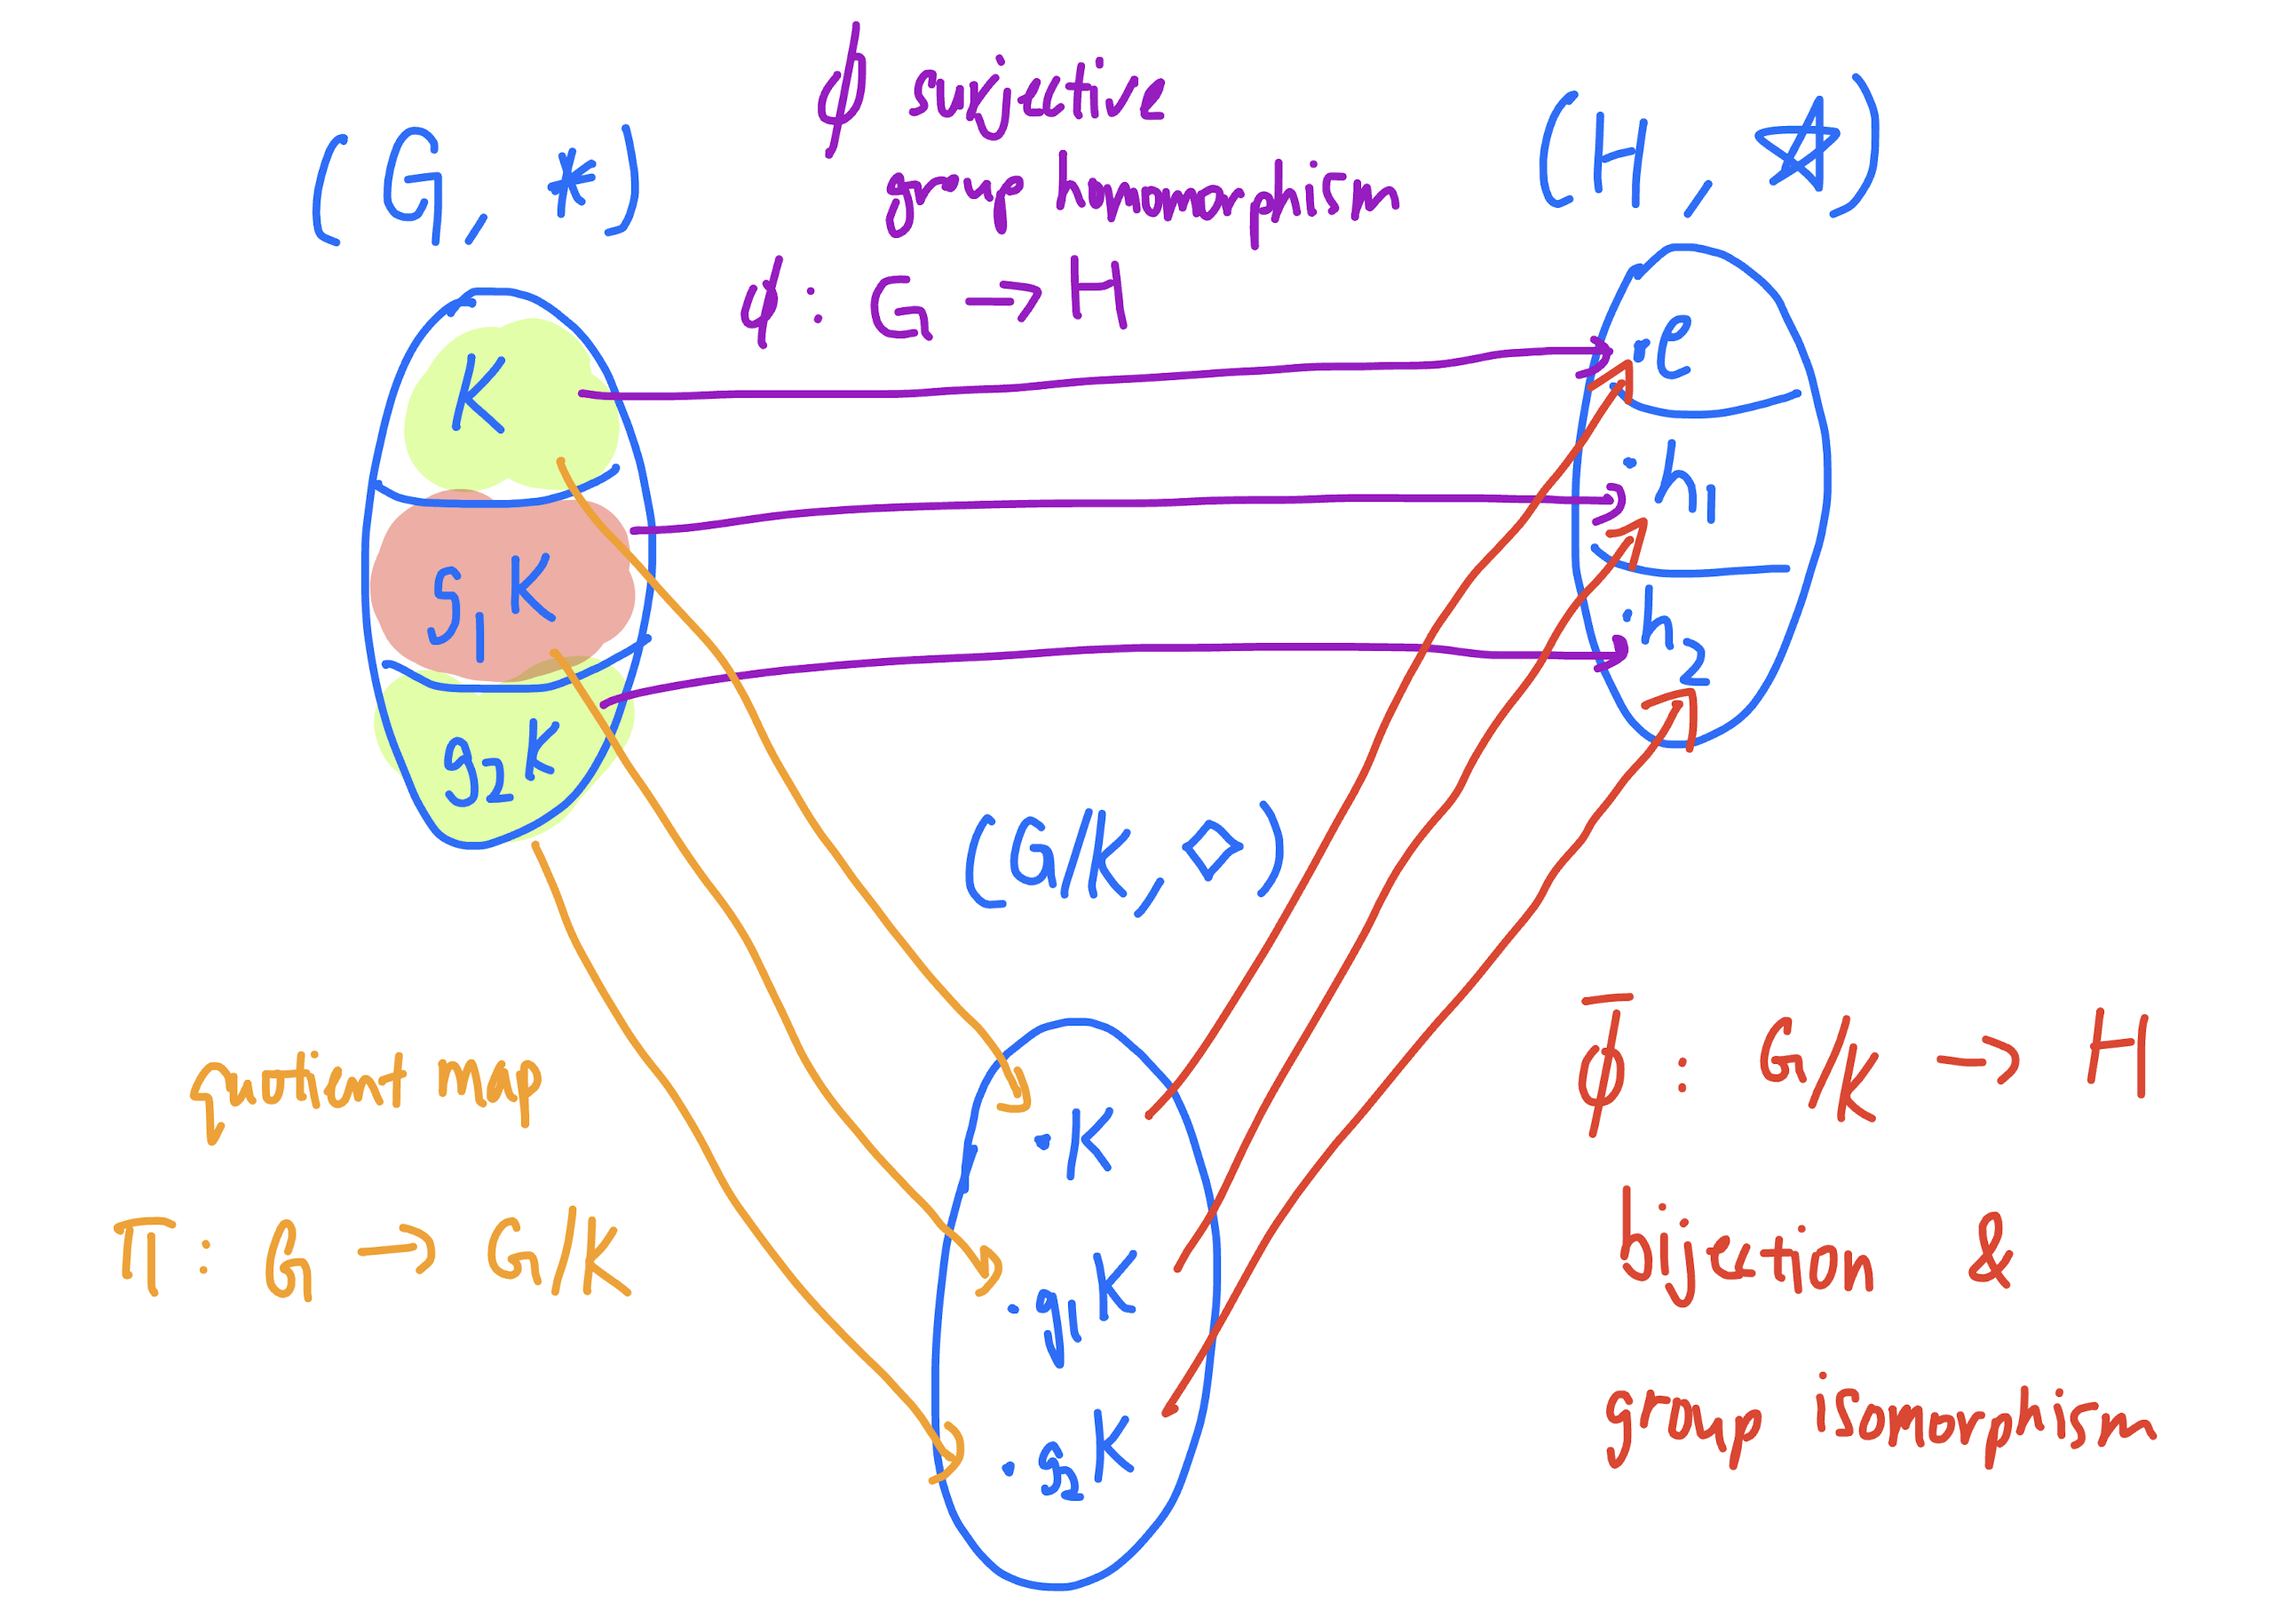
\includegraphics[width=0.8\columnwidth]{5.1}
  \end{center}
  \begin{itemize}[leftmargin=*]
    \item If $\phi$ is not surjective, then replace $H$ with the image $H' = \phi(G)$ in the definition of $\bar{\phi}$.
  \end{itemize}
  \paragraph{Corollary}
  Let $\phi: G \rightarrow H$ and $\psi: G \rightarrow H'$ be two group homomorphisms.
  \begin{itemize}[leftmargin=*]
    \item Suppose $\phi$ and $\psi$ have the same kernel $K$. Then, the images $\phi(G)$ and $\psi(G)$ are isomorphism groups.
    \item If $G$ is a finite group, then
          \[ \abs{\phi(G)} = \abs{\psi(G)} = \abs{G/K} = \abs{G} / \abs{K} \]
  \end{itemize}
  \subsection*{The Second Isomorphism Theorem} \noindent
  In this section, $G$ is a group, $M$ is a subgroup of $G$, and $K$ is a normal subgroup of $G$.
  \paragraph{Prop. 59} $MK = KM$ and it is a subgroup of $G$.
  \paragraph{Proposition 60}
  \begin{enumerate}[label=\roman*., leftmargin=*]
    \item The function $\phi: M \rightarrow MK/K$ defined by $\phi(m) = mK$ is a surjective group homomorphism.
    \item The kernel of $\phi$ is $M \cap K$. In particular, it is a normal subgroup of $M$.
  \end{enumerate}
  \subsubsection*{Second Isomorphism Theorem} \noindent
  \[ M / (M \cap K) \simeq (MK)/K \]
  \subsection*{The Third Isomorphism Theorem} \noindent
  Let $G$ be a group. Let $M$ and $K$ be normal subgroups of $G$ such that $M \supseteq K$. Then $M/K$ is a normal subgroup of $G/K$ and
  \[ (G/K) / (M/K) \simeq G/M \]
  If $M \not\supseteq K$, then replace $K$ by $M \cap K$, which is a normal subgroup of $G$ contained in $M$.
  \paragraph{Corollary} Let $M$ and $K$ be normal subgroups of $G$ such that $M \supseteq K$. Then there is a surjective group homomorphism
  \[ \phi: G/K \rightarrow G/M \]
  given by $\phi(gK) = gM$.
  \subsection*{Euler's totient function} \noindent
  Let $n$ be a positive integer. If $n = 1$, set $\Phi(1) = \{1\}$. Else set
  \[ \Phi(n) = \{x \in \Z: 0 \le x \le n, \gcd(x, n) = 1 \} \]
  \begin{itemize}[leftmargin=*]
    \item Let $*$ denote multiplication modulo $n$. Then $(\Phi(n), \ast)$ is a group.
    \item Let $\phi(n)$ denote the number of elements in $\Phi(n)$.
    \item For prime number $p$, $\Phi(p) = \{1, 2, \cdots p-1\}$, so $\phi(p) = p-1$.
    \item For prime number $p$, let $n=p^r$.
          \[ \phi(p^r) = n - \frac{n}{p} = p^r \left( 1 - \frac{1}{p} \right) = p^{r-1}(p-1) \]
  \end{itemize}
  \subsubsection*{Euler's theorem} \noindent
  Let $x$ be an integer such that $\gcd(x,n) = 1$. Then
  \[ x^{\phi(n)} \equiv 1 \pmod{n} \]
  \subsubsection*{Calculating $\phi(n)$} \noindent
  Suppose $n = p_1^{r_1} p_2^{r_2} \cdots p_n^{r_n}$. Then
  \begin{align*}
    \phi(n) & = n \left(1 - \frac{1}{p_1}\right) \left(1 - \frac{1}{p_2}\right) \cdots \left(1 - \frac{1}{p_k}\right) \\
            & = \phi(p_1^{r_1}) \phi(p_2^{r_2}) \cdots \phi(p_k^{r_k})
  \end{align*}
  \paragraph{Example} Compute $43^{866} \pmod{360}$.
  \begin{itemize}[leftmargin=*]
    \item $360 = 2^3 \cdot 3^2 \cdot 5$ so
          \[ \phi(360) = 360 \left(1 - \frac{1}{2}\right) \left(1 - \frac{1}{3}\right) \left(1 - \frac{1}{5}\right) = 96 \]
    \item Since $\gcd(43, 360) = 1$, Euler's theorem gives $43^{96} \equiv 1 \pmod{360}$.
    \item We have $866 = 96(9) + 2$ so
          \begin{align*}
            43^{866} & \equiv 43^{96(9) + 2} \equiv (43^{96})^9 43^2 \\
                     & \equiv 1^9 43^2 \equiv 49 \pmod{360}
          \end{align*}
  \end{itemize}
  \subsection*{Automorphism groups} \noindent
  Let $(G,\ast)$ be a group. An isomorphism $\phi: G \rightarrow G$ is called an automorphism of $G$. We denote the set of automorphisms of $G$ by
  \[ \Aut{G} = \{ \phi: G \rightarrow G: \phi \text{ is an isomorphism} \} \]
  \subsubsection*{Isomorphism facts}
  \begin{itemize}[leftmargin=*]
    \item Identity map $\mathrm{id}_G$ is an isomorphism.
    \item Composition of isomorphisms is an isomorphism, i.e. $\circ$ is a binary operation on $\Aut{G}$.
    \item Inverse of an isomorphism is an isomorphism.
  \end{itemize}
  \paragraph{Proposition} $(\Aut{G}, \circ)$ forms a group.
  \begin{itemize}[leftmargin=*]
    \item It is called the automorphism group of $G$.
    \item A subgroup $A$ of $(\Aut{G}, \circ)$ is called an automorphism subgroup.
  \end{itemize}
  \subsubsection*{Inner automorphism} \noindent
  Let $G$ be a group and let $g \in G$. Then $\phi_g: G \rightarrow G$ given by
  \[ \phi_g(x) = gxg^{-1} \]
  is a group automorphism. It is called an inner automorphism of $G$.
  \begin{itemize}[leftmargin=*]
    \item Let $\Inn{G} = \{ \phi_g: g \in G \}$ be the set of inner automorphisms.
    \item The subset $\Inn{G}$ is a normal subgroup of $(\Aut{G}, \circ)$.
  \end{itemize}
  \paragraph{Proposition} The map $T: G \rightarrow \Inn{G}$ given by $T(g) = \phi_g$ is a surjective group homomorphism whose kernel is the center of the group
  \[ Z(G) = \{z \in G: gz = zg \text{ for all } g \in G\} \]
  By the first isomorphism theorem,
  \[ G/Z(G) \simeq \Inn{G} \]
  \subsection*{The Sylow Theorems}
  \paragraph{Notation} Let $n$ be a positive integer. Suppose $p^e$ divides $n$, but $p^{e+1}$ does not divide $n$. We write $p^e \vv n$. Alternatively, n = $p^e m$ where $p \not\vert\; m$.
  \subsubsection*{Definition} \noindent
  Let $G$ be a finite group of order $n$. Let $p$ be a prime divisor of $n$. Let $H$ be a subgroup of order of $p^e$.
  \begin{itemize}[leftmargin=*]
    \item $H$ is called a $p$-subgroup of $G$.
    \item If $p^e \vv n$, then $H$ is called a Sylow $p$-subgroup of $G$.
  \end{itemize}
  \paragraph{Example} Let $G = S_9$. It has order $9! = 2^7 3^4 5^1 7^1$.
  \begin{itemize}[leftmargin=*]
    \item A subgroup of order $2^5$ is a 2-subgroup.
    \item A subgroup of order $2^7$ is a Sylow 2-subgroup.
  \end{itemize}
  \subsubsection*{First Sylow Theorem} \noindent
  Let $G$ be a group of order $n$. Let $p$ be a prime divisor of $n$. Then $G$ contains a Sylow $p$-subgroup.
  \paragraph{Corollary} Let $G$ be a finite group of order $n$. Let $p$ be a prime divisor of $n$. If $p^d \vert n$, then $G$ contains a subgroup of order $p^d$.
  \subsubsection*{Definition} \noindent
  Let $P$ be a subgroup of $G$. Let $g \in G$. Then $gPg^{-1}$ is a subgroup of $G$ called a conjugate of $P$. Let $P$ be a Sylow $p$-subgroup. Then a conjugate $gPg^{-1}$ is also a Sylow $p$-subgroup.
  \subsubsection*{Theorem 94} \noindent
  Let $G$ be a group of order $n$. Let $\{P_1, P_2, \cdots, P_r\}$ be all the distinct conjugates of a Sylow $p$-subgroup $P = P_1$.
  \begin{enumerate}[label=\roman*., leftmargin=*]
    \item Let $Q$ be a $p$-subgroup of $G$. Then $Q \subseteq P_i$ for some $i$.
    \item (Second) If $Q$ is a Sylow $p$-subgroup of $G$, then $Q = P_i$ for some $i$.
    \item (Third) Let $r$ denote the number of Sylow $p$-subgroups of $G$. Then
          \[ r \equiv 1 \pmod{p} \text{ and } r \vert [G:P] \]
  \end{enumerate}
  \paragraph{Corollary 95} Let $P$ be a Sylow $p$-subgroup of a finite group $G$. Then $P$ is a normal subgroup $\iff P$ is the unique Sylow $p$-subgroup of $G$.
\end{multicols*}
\end{document}
